\documentclass[15pt]{article}
\usepackage{amsmath, amsthm, amssymb, graphicx, mhchem}
\usepackage{xeCJK}
\usepackage{indentfirst}
\setlength{\parindent}{2em}
\usepackage{chemfig}
\usepackage{adjustbox}
\usepackage{multirow}
\usepackage{multicol}
\usepackage{floatrow}
\usepackage{geometry}
\usepackage{subfigure}
\usepackage[bookmarks=true, colorlinks, citecolor=blue, linkcolor=black]{hyperref}
\hypersetup{hidelinks,
	colorlinks=true,
	allcolors=black,
	pdfstartview=Fit,
	breaklinks=true}
\floatsetup{heightadjust=all, floatrowsep=columnsep}
\newfloatcommand{figurebox}{figure}[\nocapbeside][\dimexpr(\textwidth-\columnsep)/2\relax]
\newfloatcommand{tablebox}{table}[\nocapbeside][\dimexpr(\textwidth-\columnsep)/2\relax]

\title{CNN History}
\author{Jingru Men}
\date{\today}
\linespread{1.5}

\begin{document}

\maketitle
\tableofcontents
\section{概述}
对于图形所做的数据分析,如识别、分割等,其发展历程在2012年有一个史诗级的进步,就是因为卷积神经网络(Convolutional Netural Network,以下简称CNN)的引入和同时期硬件GPU算力的急速发展。但是CNN并不是在2012年才提出的,也并非只应用于图形的数据分析,CNN在1D数据处理上的应用和传统的2D处理图像,乃至如今3D处理拥有上下文关系的体积或视频的应用息息相关。Cnn网络在不同维度和不同场景有着不同的应用形式。如2d-cnn的深度模型拥有大量参数,抽象能力高,且对提取到的特征有区域识别的需求。1d-cnn的深度模型不需要很深,因为计算复杂度低且参数量相对较少,且要求实时性核可部署在计算能力低的设备中。3d-cnn的参数量更巨,对特征提取的要求更高,也更注重时间维度和空间维度的上下文关系。Cnn的发展成熟始于2d,故在1d和3d应用中有结构的类比关系和针对场景做出的特别改进。本文以2d-cnn的发展和改进原理为基础,介绍cnn在不同维度的应用差异和模型结构。

结构:本文在1中依照时间线介绍2d-cnn的早期发展,2中为2015年后以resnet系列模型的改进,3 介绍了其他多种模型的改进思路。4,5中分别介绍1d-cnn和3d-cnn在不同场景下的应用,着重介绍医疗图像场景下的应用。(3d部分择文另写) 

\section{2d-cnn的改进和发展}
\subsection{卷积神经网络的初创时期}
在卷积神经网络出现之前,是有一个人工神经网络的时期的。神经网络这个概念出现的很早,早在上世纪40年代,随着解剖学和脑神经学的发展,人们就开始考虑仿造大脑的基本结构——神经元来构建人工智能的想法了。

人工神经网络是一种模仿生物神经网络的数学抽象,而人工神经元是其基本单位。1943年,第一个人工神经元模型的提出者是McCulloch和Pitts[1],他们的M-P神经元模型很简单,如图1所示,单个神经元有三个树突接口[2],其他神经元的输出由树突触接入,输入的信号经过细胞核处的某种运算(这里使用的是加权求和),如果运算结果大于某一阈值,则激活一个脉冲(动作电势)作为输出,输出也会分为许多小分支携带相同信息作为下一个神经元的树突输入接口。整体数学过程如公式(1)所示。如此,一个仿生的人工神经元的数学模型就完成了。这是一个“婴儿”神经元,但它却是后面一切深度学习CNN的理论基础和数学基础。由人工神经元组成的神经网络就被称为人工神经网络ANN(Artificial Neural Network)。1949年Danald Olding Hebb的赫布学习率的出现,说明了学习行为与神经元的联系,机器学习行为的可能性所需的一切零件便都具备了。


\section{Data Analysis}
This is the raw data of the experiment. It records the length value for positions of resonance.
\begin{table}[H]
\begin{tabular}{|c|c|c|}
\hline
Frequency $f$ (Hz) $\pm 1$ & First maximum loudness $L_1$ (mm) $\pm 0.5$ & Second maximum loudness $L_2$ (mm) $\pm 0.5$ \\ \hline
860                        & 40                                          & 223                                          \\ \hline
1200                       & 93                                          & 170                                          \\ \hline
1500                       & 99                                          & 232                                          \\ \hline
\end{tabular}
\caption{Raw data}
\end{table}

The we can calculate the wavelength $\lambda$ and sound speed $v$ through the following formula:
$$\lambda=(L_2-L_1) \cdot 2$$
$$v=f \cdot \lambda$$

\begin{table}[H]
\begin{tabular}{|c|c|c|c|}
\hline
Frequency $f$ (Hz) $\pm 1$ & Wavelength $\lambda$ (m) $\pm 0.001$ & Sound speed $v$ (m/s) & Uncertainty of sound speed (m/s) \\ \hline
860                        & 0.366                                & 315                   & 1.23                             \\ \hline
1200                       & 0.154                                & 185                   & 1.35                             \\ \hline
1500                       & 0.266                                & 399                   & 1.77                             \\ \hline
\end{tabular}
\centering
\caption{Wavelength and sound speed}
\end{table}

\noindent e.g. $\lambda_1=(223 \cdot 10^{-3}m-44 \cdot 10^{-3}m) \cdot 2=0.366m$

$\Delta \lambda=\Delta L_1+\Delta L_2=0.5mm+0.5mm=0.001m$

$v_1=f_1 \cdot \lambda_1=860Hz \cdot 0.366m \approx 315m/s$

$\Delta v_1=315m/s \cdot (\dfrac{0.001m}{0.366m}+\dfrac{1Hz}{860Hz}) \approx 1.23m/s$

Then, we calculate the average sound speed and the percentage difference between the experimental sound speed and the actual sound speed $343m/s$.
$$v_{average}=\dfrac{315+185+399}{3} \approx 300m/s$$
$$\% Difference=\dfrac{v_{average}-343m/s}{343m/s} \approx -12.7\%$$

\subsection{Graph}
This is the graph of the vernier during the experiment.
\begin{figure}[H]
    \centering
    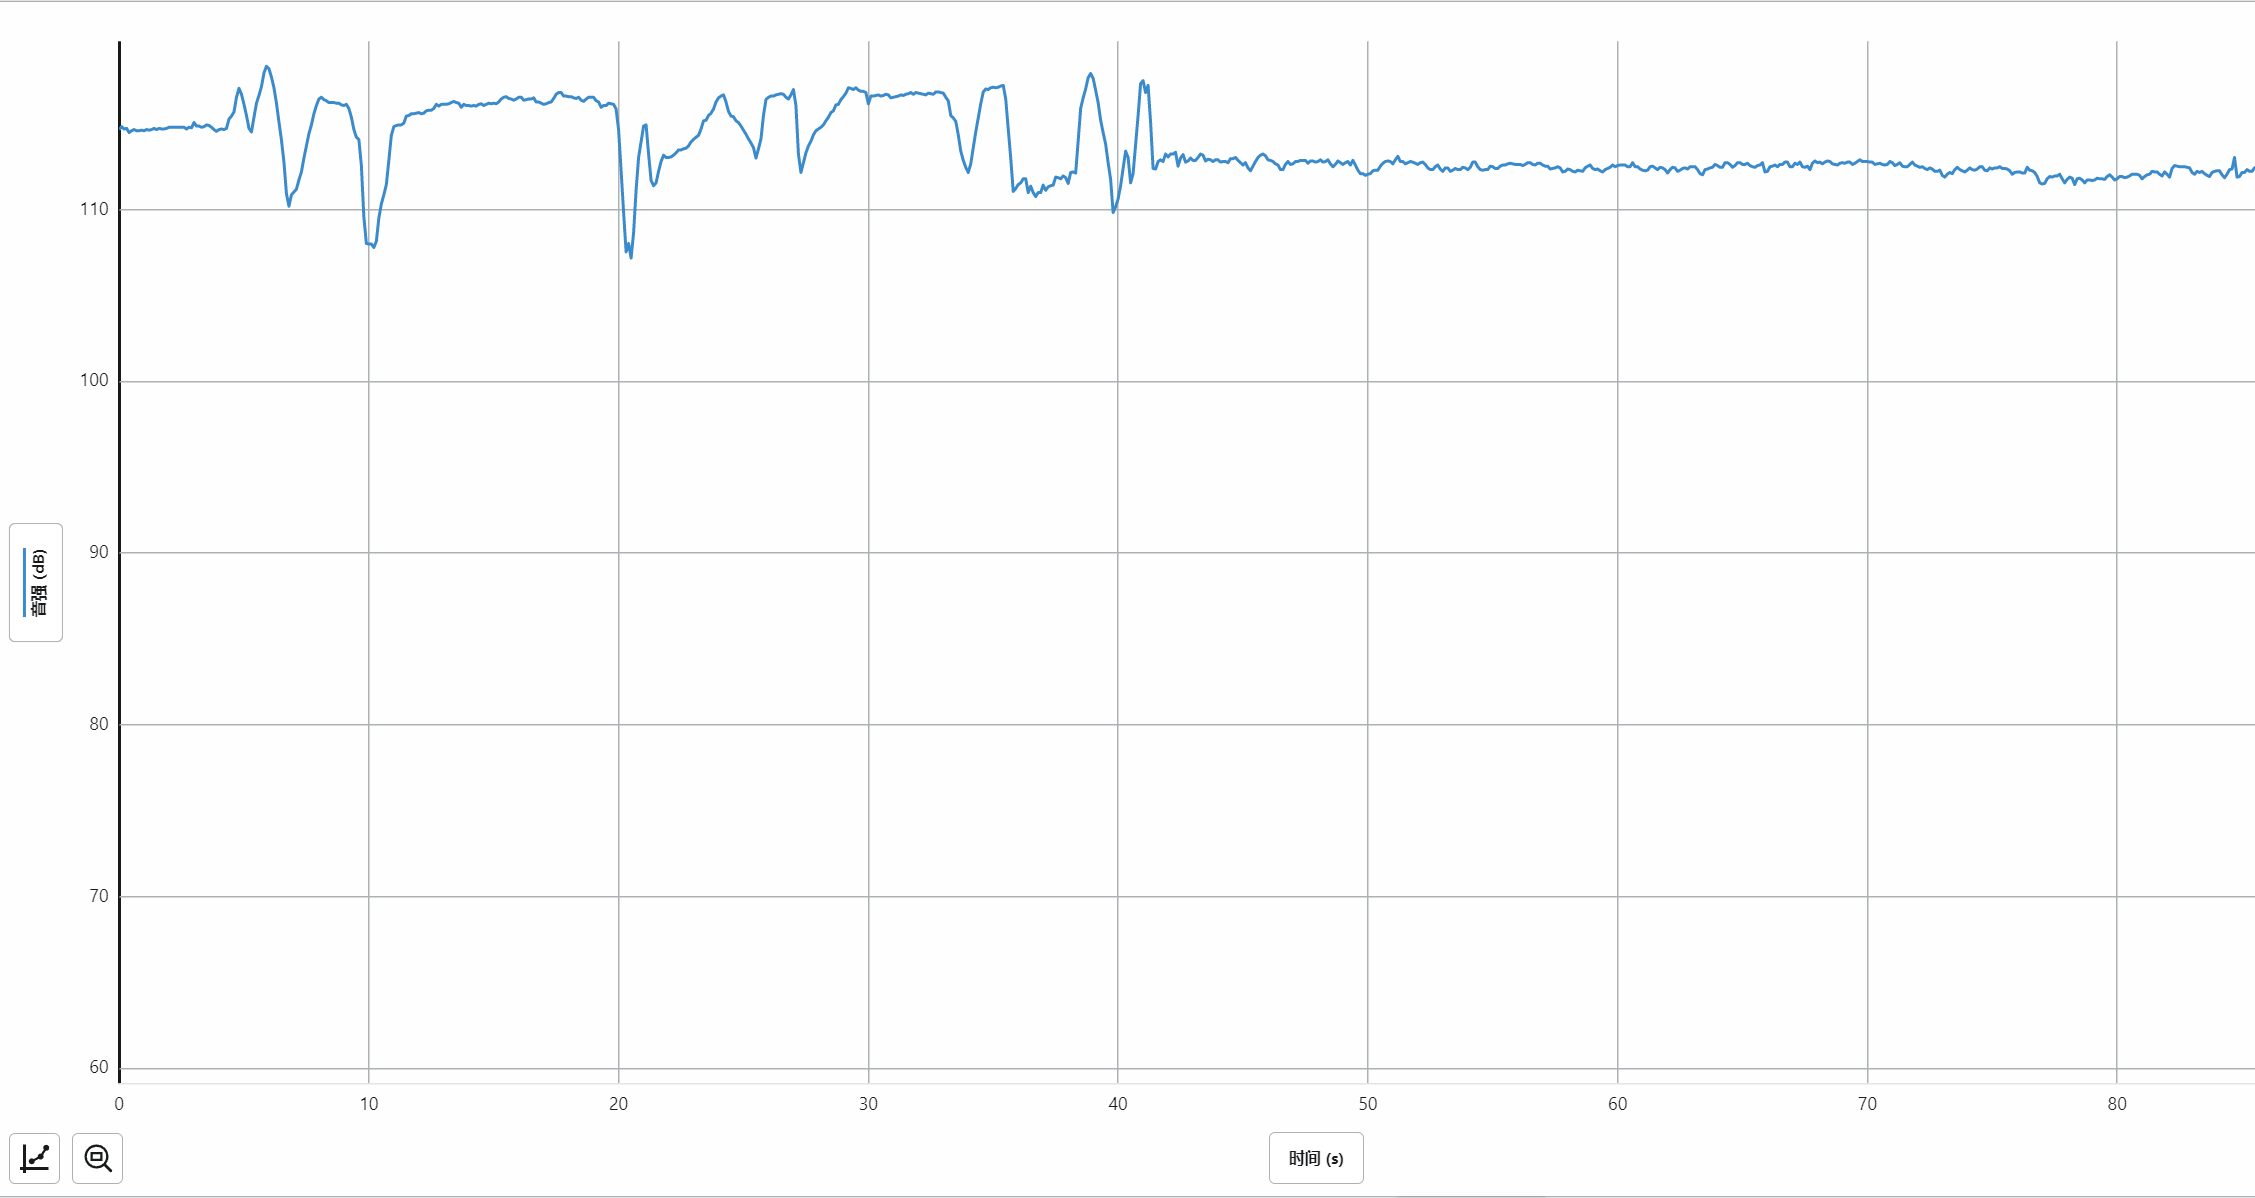
\includegraphics[width=0.75\textwidth]{sound intensity-time graph.png}
    \caption{Sound intensity-Time graph}
\end{figure}

\section{Conclusion}
Based on the data collected and calculations made, we can conclude that the speed of sound in the air was measured by using standing waves and was found to be $315m/s$, $185m/s$, and $399m/s$, with an average of $300m/s$. However, the percentage difference between the experimental sound speed and the actual sound speed of 343 m/s was found to be quite high at about -12.7\%.

The reason for such high percentage differences could be due to various factors such as experimental errors, uncertainties in measurements, and limitations of the equipment used. One of the major sources of error in this experiment could be the difficulty in accurately measuring the distance between two antinodes of the standing waves. Additionally, the experimental setup may not have been completely free from external noise and disturbances, which could have affected the accuracy of our results.

To reduce such errors and improve the accuracy of our results, we can improve the experimental setup by using better-quality equipment and ensuring that the setup is completely isolated from external noise and disturbances.

\end{document}
